\chapter{Project Oversight}
\label{vl:tc-project}


\Dword{tc} is responsible for technical quality and the schedule but
not for consortia funding or budgets.  \Dword{tc} will try to resolve
any issues it can but will likely push all financial issues to the
\dword{tb}, \dword{exb} and \dword{rcoord} for resolution.

\Dword{tc} maintains a web
page\footnote{\url{https://web.fnal.gov/collaboration/DUNE/DUNE\%20Project/\_layouts/15/start.aspx\#/}.}
with links to project documents. \Dword{tc} also maintains
repositories of project documents and drawings. These include the
\dword{wbs}, schedule, risk register, requirements, milestones,
strategy, detector models and drawings that define the \dword{dune}
detector.

The following sections describe the systems that track the progress of
the \dword{dune} project as well as the ways in which this large,
distributed organization is managed.

%%%%%%%%%%%%%%%%%%%%%%%%%%%%%%%%
\section{Schedule}
\label{sec:fdsp-coord-controls}

A series of tiered milestones have been developed for the \dword{dune}
project. The spokespersons and host laboratory director are
responsible for the tier 0 milestones. Three tier 0 milestones have
been defined and the dates set:
\begin{enumerate}
\item Start main cavern excavation \hspace{2.58in} 20xx
\item Start \dword{detmodule}~1 installation \hspace{2.1in} 20xx
\item Start operations of \dwords{detmodule} \#1--2 with beam \hspace{0.8in} 20xx
\end{enumerate}
These dates will be revisited this spring before the \dword{tdr} is reviewed. The
\dword{tcoord} and \dword{lbnf} project manager hold the Tier 1
milestones; these milestones will be defined in advance of the
\dword{tdr} review. The consortia themselves hold the Tier 2
milestones.

Table~\ref{tab:DUNE_schedule} provides a high level version of the
\dword{dune} milestones from the \dword{ims}.
\begin{dunetable}
  [Overall \dword{dune} Project Tier-1 milestones.]
  {p{0.84\linewidth}p{0.14\linewidth}}
  {tab:DUNE_schedule}
  {Overall \dword{dune} Project Tier-1 milestones.}
  Milestone & Date   \\ \toprowrule
  RRB Approval of Technical Design Review                       &  \\ \colhline
  Beneficial Occupancy of Integration Test Facility             &  \\ \colhline
  Construction of steel frame for Cryostat \#1 complete         &  \\ \colhline
%  Construction of Mezzanine for Cryostat \#1 complete           & 01/17/2022 \\ \colhline
%  Begin integration/testing of Detector \#1 components at ITF   & 02/01/2022 \\ \colhline
  Beneficial Occupancy of Central Utility Cavern Counting room  &  \\ \colhline
  Construction of steel frame for Cryostat \#2 complete         &  \\ \colhline
%  Construction of Mezzanine for Cryostat \#2 complete           & 08/01/2022 \\ \colhline
  \textbf{Beneficial occupancy of Cryostat \#1}                 & \textbf{} \\ \colhline
  Cryostat \#1 ready for TPC installation                       &  \\ \colhline
%  Begin integration/testing of Detector \#2 components at ITF   & 11/01/2023 \\ \colhline
  \textbf{Beneficial occupancy of Cryostat \#2}                 & \textbf{} \\ \colhline
%  Begin closing Temporary Construction Opening for Cryostat \#1 & 05/01/2024 \\ \colhline
  Cryostat \#2 ready for TPC installation                       &  \\ \colhline
  Cryostat \#1 ready for filling                                &  \\ \colhline
%  Begin closing Temporary Construction Opening for Cryostat \#2 & 07/18/2025 \\ \colhline
  \textbf{Detector \#1 ready for operations}                    & \textbf{} \\ \colhline
  Cryostat \#2 ready for filling                                &  \\ \colhline
  \textbf{Detector \#2 ready for operations}                    & \textbf{} \\
\end{dunetable}
To monitor progress, \Dword{tc} will maintain the \dword{ims} that
links all consortium schedules and contains milestones for each
consortia.  The schedules will go under change control after each
consortium agrees to the milestone dates and the \dword{tdr} is
approved.  In addition to the overall \dword{ims} for construction and
installation, a schedule of key consortia activities has been
developed during 2018 and 2019.

To ensure that the \dword{dune} detector remains on schedule,
\dword{tc} will monitor schedule status from each consortium and organize
reviews of schedules and risks as appropriate.  As schedule problems
arise, \dword{tc} will work with affected consortium to resolve the
problems. If problems cannot be solved, the \dword{tc} will take the issue to the
\dword{tb} and \dword{exb}.

A monthly report with input from all consortia will be published by
\dword{tc}. This will include updates on consortium and \dword{tc}
technical progress against the \dword{ims}.

%%%%%%%%%%%%%%%%%%%%%%%%%%%%%%%%
\section{Risks}
\label{sec:fdsp-coord-risks}

\fixme{new standard risks table for autogenerating latex as of 3/25. I will send email. Anne}

\dword{dune} has implemented a risk registry in DocDB-6443. This
document includes tabs for consortia risks and \dword{tc} risks. It
includes a summary tab for the most significant overall \dword{dune}
risks. Tables~\ref{fig:dune_risks1} and~\ref{fig:dune_risks2} show the
overall \dword{dune} risks. This registry is updated approximately
every year. The last update was in early 2018 before ProtoDUNE was completed and the next update is
planned for spring 2019. In the next update, several risks associated
with ProtoDUNE will be retired.
\begin{dunefigure}[\dword{dune} overall risk register]{fig:dune_risks1}
  {First page of \dword{dune} overall risk register.}
  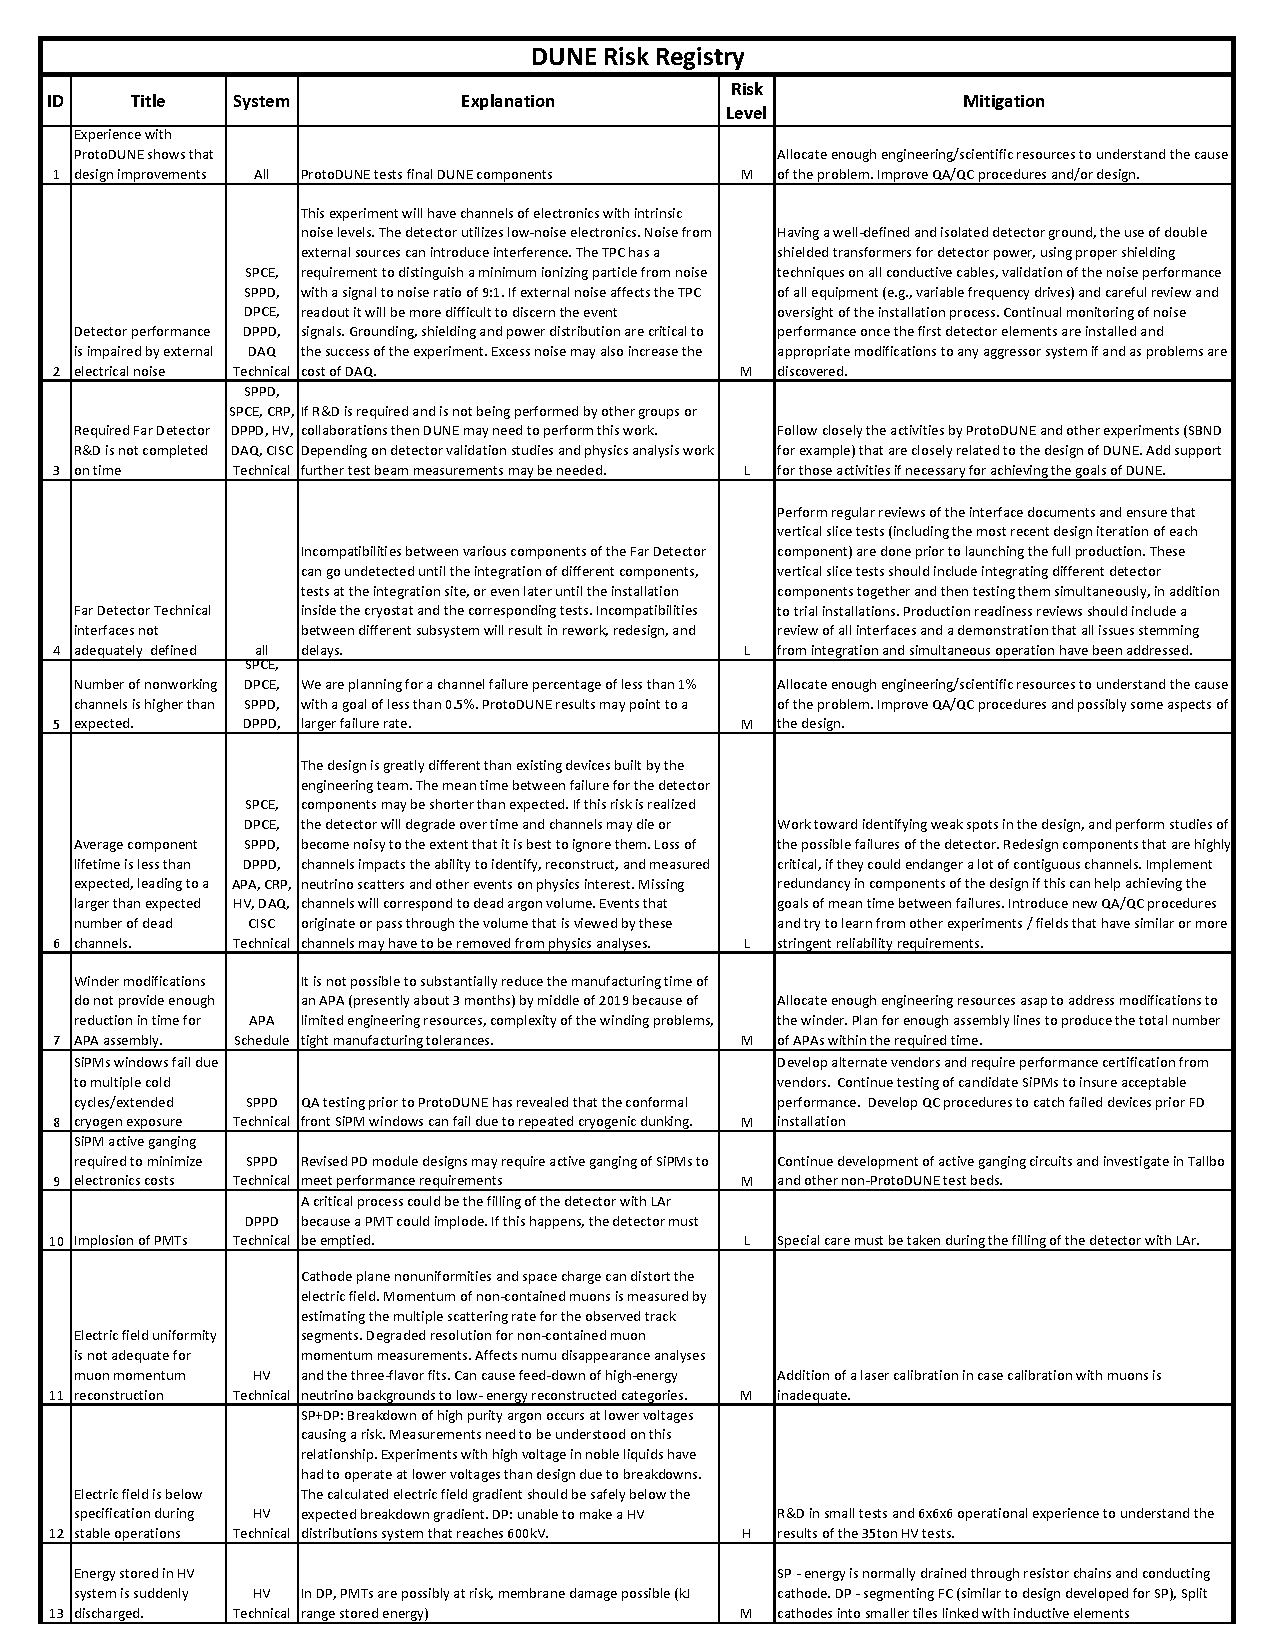
\includegraphics[width=0.99\textwidth]{DUNE_Risks_v4b1}
\end{dunefigure}
\begin{dunefigure}[\dword{dune} overall risk register]{fig:dune_risks2}
  {Second page of \dword{dune} overall risk register.}
  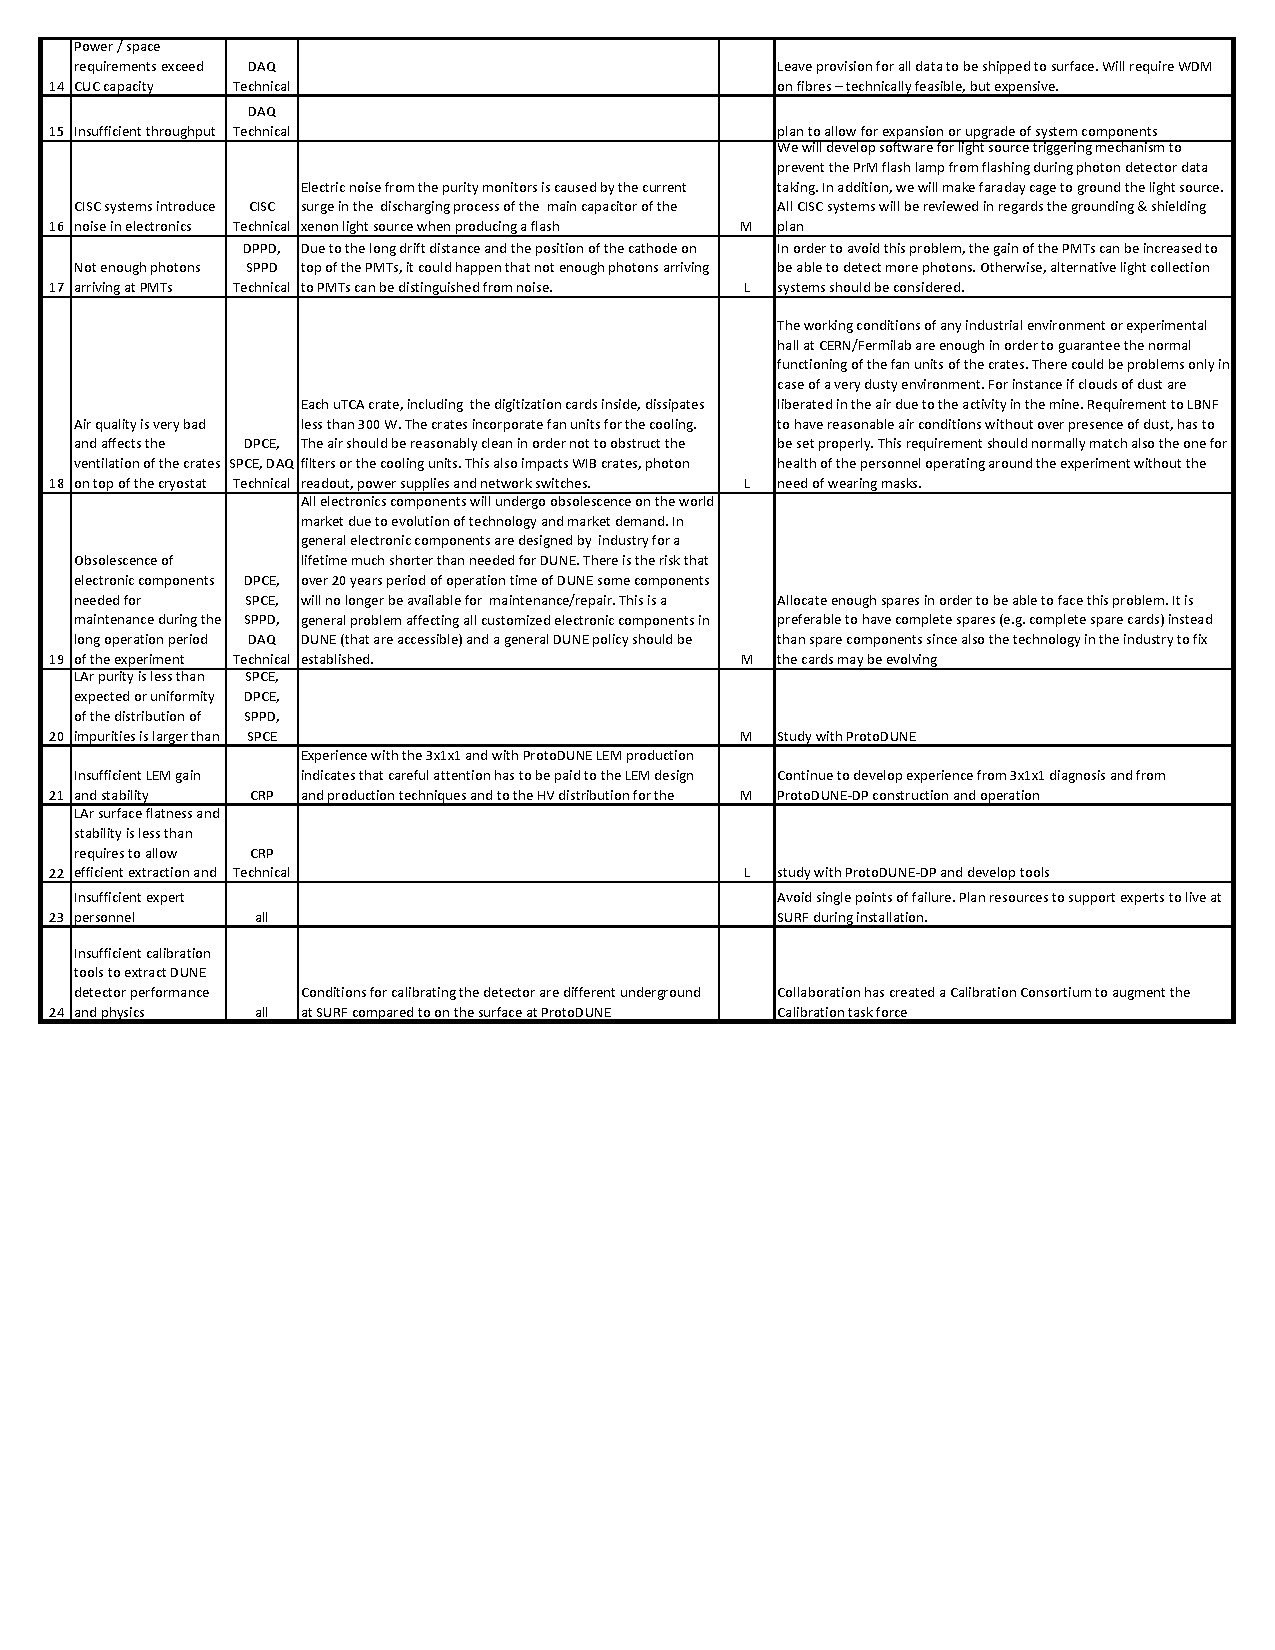
\includegraphics[width=\textwidth]{DUNE_Risks_v4b2}
\end{dunefigure}
\dword{lbnf} and \dword{dune}-US would like \dword{dune} to update and
expand this risk register to allow a Monte Carlo analysis of cost and
schedule risks to the \dword{us} project resulting from international
\dword{dune} risks. This request is under consideration.

One update to the risk registry has been for \dword{tc}, in which some
risks  associated with  DUNE  integration and  installation have  been
added. Table~\ref{fig:tc_risks} summarizes the \dword{tc} risks.
\begin{dunefigure}[\dword{tc} risks]{fig:tc_risks}
  {\dword{tc} risk register.}
  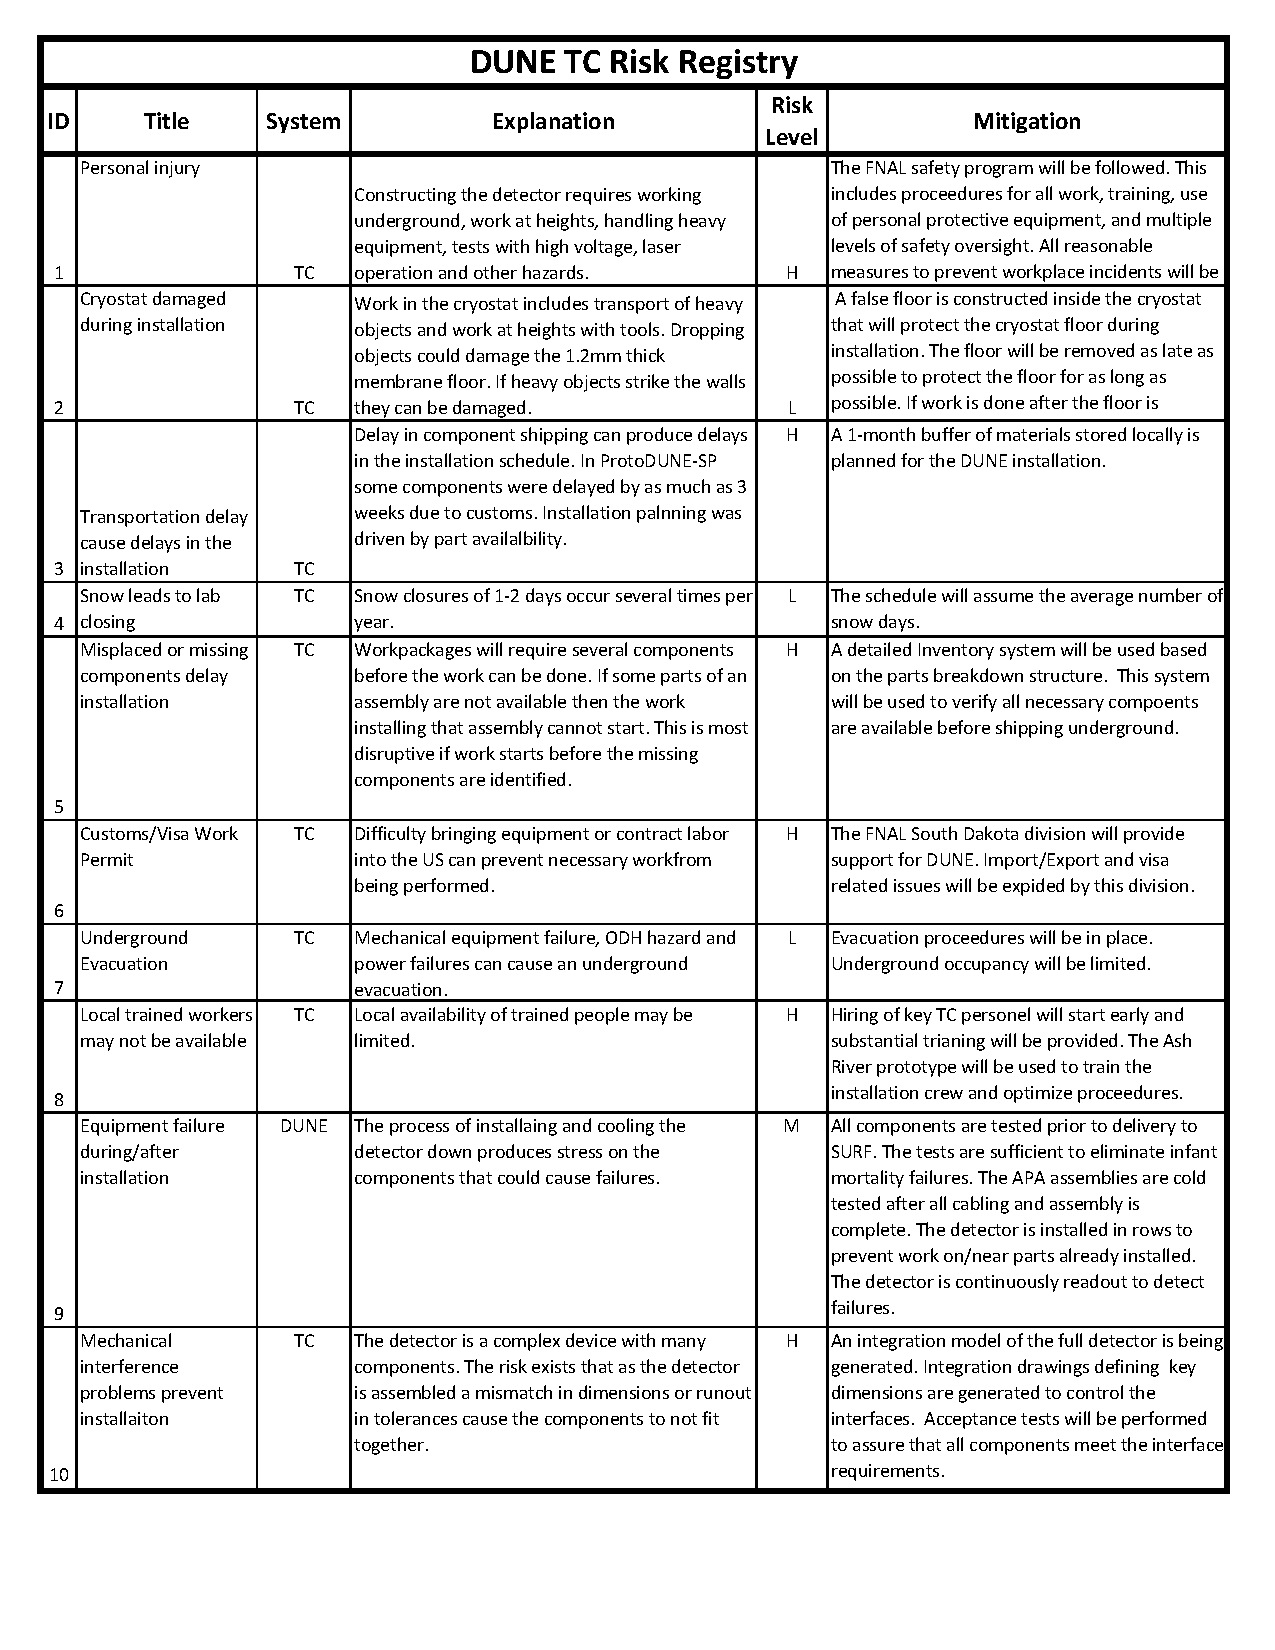
\includegraphics[width=\textwidth]{TC_Risks_v4b}
\end{dunefigure}

The next update of the risk register will separate the current overall
risk level into separate quantified probability and impact.

Successfully operating \dword{protodune} retires many
potential risks in \dword{dune} itself. This includes most risks associated with the
technical design, production processes, \dword{qa}, integration
and installation. Residual risks remain relating to design and
production modifications associated with scaling to \dword{dune}, mitigations
to known installation and performance issues in \dword{protodune}, underground
installation at \surf and organizational growth.

The highest technical risks include development of a system to
deliver \SI{600}{kV} to the \dual cathode; general delivery of the
required \dword{hv}; cathode and \dword{fc} discharge to the cryostat
membrane; noise levels, particularly for the \dword{ce}; %cold TPC electronics,
number of dead channels; lifetime of components surpassing \dunelifetime{}; %20 years,
\dword{qc} of all components; verification of improved \dword{lem}
performance; verification of new cold  \dword{adc} and  \dword{coldata} performance;
argon purity; electron drift lifetime; \phel light yield;
incomplete calibration plan; and incomplete connection of design to
physics. Other major risks include insufficient funding, optimistic
production schedules, incomplete plans for integration, testing and installation.

Key risks for \dword{tc} to manage include the following:
\begin{enumerate}
\item Consortia leave too much scope unaccounted for and too much falls
  to  the \dword{comfund}.
\item Insufficient organizational systems are put into place to
  ensure that this complex international mega-science project,
  including \dword{tc}, \fnal as host laboratory, \surf, DOE, and all international
  partners continue to work together successfully to ensure
  appropriate processes and services are provided for the success of
  the project.
\item Inability of \dword{tc} to obtain sufficient personnel resources to
  ensure that \dword{tc} can oversee and coordinate all project tasks.  While the \dword{us}, 
  as host country, has a special responsibility to \dword{tc}, personnel resources should
  be directed to \dword{tc} from each collaborating country. 
\end{enumerate}

The consortia have provided preliminary versions of risk analyses that
have been collected on the \dword{tc} webpage (DocDB-6443). These have
been developed into an overall risk register that will be monitored
and maintained by \dword{tc} in coordination with the consortia.  The
next update of the risk register is planned for spring 2019, in
advance of the final \dword{tdr} submission.

%%%%%%%%%%%%%%%%%%%%%%%%%%%%%%%%
\section{Requirements}
\label{sec:fdsp-coord-requirements}

The scientific goals of \dword{dune} as described in \dword{dune}
\dword{tdr} Volume~\volnumberexec:~\voltitleexec include
\begin{itemize}
\item a comprehensive program of neutrino oscillation measurements
  including the search for CP violation
\item measurement of $\nu_{e}$ flux from a core-collapse supernova within our
  galaxy should one occur during \dword{dune} operations
\item searching for baryon number violation
\end{itemize}
These goals motivate a number of key detector requirements: drift
field, electron lifetime, system noise, photon detector light yield
and time resolution. The \dword{exb} has approved a list of high
level detector specifications, including those listed above. These are
maintained in edms-xxxx, and the high level requirements with
significant impact on physics are highlighted in
Table~\ref{tab:dunephysicsreqs}.
\begin{dunetable}
  [\dword{dune} physics-related specifications owned by \dword{exb}]
  {p{0.025\textwidth}p{0.06\textwidth}p{0.2\textwidth}p{0.35\textwidth}p{0.15\textwidth}p{0.1\textwidth}}
  {tab:dunephysicsreqs}
  {\dword{dune} physics-related specifications owned by \dword{exb}}
  ID & System & Parameter & Physics Requirement Driver & Requirement & Goal \\ \toprowrule
  1   & HVS    & Minimum drift field &  Limit recombination, diffusion and space charge impacts on particle ID. Establish adequate \dword{s/n} for tracking. & >\SI{250}{V/cm} & \spmaxfield \\ \colhline
  2   & CE     & System noise & The noise specification is driven by pattern recognition and two-track separation.  & <\SI{1000}{enc} & ALARA \\ \colhline
  3   & PDS    & Light yield  & The light yield shall be sufficient to measure time of events with visible energy above 200 MeV.  Goal is 10\% energy measurement for visible energy of 10 MeV.  & >\SI{0.5}{pe/MeV} & >\SI{5}{pe/MeV}  \\ \colhline
  4   & PDS    & Time resolution  & The time resolution of the photon detection system shall be sufficient to assign a unique event time.  & $<\,\SI{1}{\micro\second}$ & $<\,\SI{100}{\nano\second}$  \\ \colhline
  5   & all    & liquid argon purity & The LAr purity shall be sufficient to enable drift e- lifetime of 3 (10)ms & $<$\,\SI{100}{ppt} & $<$\,\SI{30}{ppt} \\ \colhline
\end{dunetable}
Eleven other significant specifications owned by the \dword{exb} are
listed in Table~\ref{tab:dunephysicsspecs} along with another twelve
high level engineering specifications.
\begin{dunetable}
  [\dword{dune} physics-related specifications owned by \dword{exb}]
  {p{0.025\textwidth}p{0.06\textwidth}p{0.2\textwidth}p{0.35\textwidth}p{0.15\textwidth}p{0.1\textwidth}}
  {tab:dunephysicsspecs}
  {\dword{dune} high level system specifications owned by \dword{exb}}
  ID & System & Parameter & Physics Requirement Driver & Requirement & Goal \\ \toprowrule
  6   & APA & Gaps between APAs  & minimize events lost due to vertex in gaps between APAs (15mm on same support beam, 30mm on adjacent beams) & <\SI{30}{mm} & <\SI{15}{mm} \\ \colhline
  7   & DSS & Drift field uniformity & tolerance on drift field due to component location & $<\,\SI{1}{\%}$  &   \\ \colhline
  8   & APA & wire angles  & 0$^\circ$ collection, $\pm$35.7$^\circ$ induction &  &  \\ \colhline
  9   & APA & wire spacing  & \SI{4.669}{mm} for U,V; \SI{4.790}{mm} for X,G &  &  \\ \colhline
  10  & APA & wire position tolerance  & & $\pm\,\SI{0.5}{mm}$  &  \\ \colhline
  11  & HVS & Drift field uniformity & tolerance on drift field due to HVS system & $<\,\SI{1}{\%}$  &  \\ \colhline
  12  & HVS & Cathode power supply ripple & very small compared to intrinsic electronics noise & $<\,\SI{100}{enc}$ &   \\ \colhline
  13  & CE & Frontend peaking time  & optimize vertex resolution & \SI{1}{\micro\second} &  \\ \colhline
  14  & CE & Signal saturation  & largest signals occur with multiple protons in the primary vertex & 500k $e^-$ &  \\ \colhline
  15  & cryo & LAr N$_2$ contamination  & optical attenuation length in liquid argon with 50~ppm of N$_2$ contamination is roughly 3~m & $<\,\SI{25}{ppm}$ &  \\ \colhline
  16  & all & Detector dead time  & risk of missing a supernova burst if all operating cryostats are offline & $<\,\SI{0.5}{\%}$ &  \\ \colhline
\end{dunetable}
The high level \dword{dune} requirements that drive the \dword{lbnf} design are
maintained in DocDB-112 and under change control. These are owned by
the \dword{dune} \dword{tc} and the \dword{lbnf} project manager.

Lower level detector specifications are held by the consortia and
described in the \dword{dune} \dword{tdr} \dword{dsp}
Volume~\volnumbersp\ and \dword{ddp} Volume~\volnumberdp\ chapters for
each consortium. A complete list of detector specifications is
provided in Chapter~\ref{ch:tc-sp-reqs}.

\section{Reviews}
\label{vl:tc-review}

The \dword{tc} reviews all stages of detector development and works
with each consortium to arrange reviews of the design (\dword{cdrev},
\dword{pdr} and \dword{fdr}), production (\dword{prr} and
\dword{ppr}) and \dword{orr} of their system.  These reviews provide
information to the \dword{tb} to help in evaluating technical
decisions.  Review reports are tracked by \dword{tc} and provide
guidance on the key issues that require engineering oversight by the
\dword{tc} engineering team. \Dword{tc} maintains a calendar of
\dword{dune} reviews.

\Dword{tc} works with consortia leaders to review all detector
designs.  As part of the \dword{tdr} development \dwords{pdr} are
planned for each subsystem in advance of the \dword{tdr} followed by
\dwords{fdr} after the \dword{tdr}.  All major technology decisions
will be reviewed before down-select.  \Dword{tc} may form task forces
as needed to address specific issues that require more in depth
review.


Producing detector elements begins only after
successful \dwords{prr}. Regular production progress
reviews will be held once production starts. The \dwords{prr}
will typically include a review of the production of \textit{Module 0}, the
first module produced at the facility. \Dword{tc} will work with
consortia leaders on all production reviews.

\Dword{tc} coordinates technical documents for the LBNC
technical design review.

The review process is an important part of the \dword{dune} QA process
as described in Section~\ref{sec:verification}, both for
design and production.

The review process has been in place since 2016 with various reviews
of \dword{protodune} components and has continued into the first \dword{dune}
reviews in 2018. Past reviews and scheduled reviews are in the
\dword{dune} Indico at https://indico.fnal.gov/category/586.
Review reports are in DocDB-1584.

\subsection{Design Reviews}

The \dword{dune} design review process is described in DocDB-9664
and is consistent with the \fnal review process described in
http://eshq.fnal.gov/manuals/feshm. Design reviews for \dword{protodune} were held for each
major system. Because the schedule was extremely tight for \dword{protodune}, only a single design review
was held for each system.

The successful operation of \dword{protodune} means \dword{dune} is at
a very advanced state of design. The strategy goiong forward is to
hold \dword{cdrev} for systems with significant changes from
\dword{protodune}. These systems include the \dword{dss}, \dword{pds} and
\dword{daq}. All systems will go through \dword{pdr} to review
design changes from \dword{protodune} and \dword{fdr} after the
\dword{tdr}.

\dword{tc} has established an Engineering Safety Committee with
mechanical and electrical engineering experts from collaborating
institutions to develop processes and procedures to evaluate engineering designs using accepted international safety
standards. The current status of international code equivalencies is
discussed further in Section~\ref{sec:esh_codes}. The codes and
standards to which each system is designed will be reviewed as part of
the \dword{pdr} and \dword{fdr}.

\subsection{Production Reviews}

Once the designs are finished, production reviews will be held
before significant funds are authorized for large production
runs. These reviews are closely coordinated with the QA team. The
expectation is that a module 0 be produced and presented as part of the \dword{prr}.

Once production has started, \dword{tc} will schedule \dword{ppr}
as appropriate to monitor production schedule and quality.

\subsection{Operations Reviews}

Operation readiness reviews (
http://eshq.fnal.gov/manuals/feshm/\#series2000) are the final safety
check out before equipment can be operated.

\subsection{Review Tracking}

Tracking and controling review recommendations is part of the review
process. Later review committees assess recommendations from earlier reviews. \dword{tc} assures that
the consortia respond to review recommendations and 
works with the consortia to make sure the responses are appropriately documented and
implemented. Reports from \dword{dune} reviews are maintained in
DocDB-1584 along with the list of recommendations.


%%%%%%%%%%%%%%%%%%%%%%%%%%%%%%%%
\section{Lessons Learned}
\label{sec:fdsp-coord-lessons}

A detailed list of lessons learned from construction and operation of
\dword{pdsp} is in DocDB-8255. These lessons have driven planning for
\dword{dune} and have led to some design changes in
\dword{dune}. Lessons learned will continue to be updated throughout
the final design stage and into production. The methodologies are
described in Section~\ref{sec:lessons_learned}.


%%%%%%%%%%%%%%%%%%%%%%%%%%%%%%%%
\section{Reporting}
\label{sec:fdsp-coord-reporting}

The \dword{dune} project has published regular monthly reports since
the final design and construction of \dword{protodune} began in
earnest in summer 2016. \Dword{tc} will continue to compile and publish these
reports. Reporting will expand to include monthly reports against the
\dword{ims}. The \dword{dune} project provides regular reports to the
LBNC at reviews several times a year. The \dword{dune} project
produces reports from design, production and operations reviews.

